\documentclass[xelatex,ja=standard,jafont=noto]{bxjsarticle}
\usepackage[utf8]{inputenc}

\date{Oct.13 2020}

\usepackage{natbib}
\usepackage{graphicx}
\usepackage{tikz}
\usepackage{circuitikz}
\usepackage{tabularx}
\usepackage{diagbox}
\usepackage{amsmath,amssymb}
\usepackage{hyperref}


\begin{document}


	\begin{titlepage}
			\begin{center}
				
				{\Large 令和2年}
				
				\vspace{10truept}
				
				{\Large 機械工学実験2}
				
				\vspace*{140truept}
				
				{\Huge モータ特性プリレポート} 
				
				\vspace{160truept}
				
				{\Large 指導教員}
				
				\vspace{10truept}
				
				{\Large Iizuka Kojiro}
				
				\vspace{70truept}
				
				{\Large 芝浦工業大学}
				
				\vspace{10truept}
				
				{\Large 機械制御システム}
				
				\vspace{30truept}
				
				{\Large bq18026 関宇}      
				
			\end{center}
		\end{titlepage}





\section{課題1}

DC サーボモータの仕組みについて調べて説明してください(サーボとはどのようなものか,DC モータの構造とエンコーダの仕組みに分けて説明してください).\\

\subsection{DCモータ系の構造$ ^{[1]} $}

DCモータは,電気的な入力(電流や電圧)によって,機械的な出力,つまり,回転角や回転速度を得るものである.\\

\begin{figure}[h!]
    \centering
    \includegraphics[scale=0.75]{012.png}
    \caption{DCモータの構造 }
\end{figure}


磁界中に導線が置かれ,導線に電流が流れると導線には力が動く.直流モータの回転力はこの導線に動く力によって発生し,フレミングの左手の法則に従う.回転する部分をロータ(rotor),回転力を発生するための導線を電機子(armature)と呼び,電源から電流を電機子に注入する部分をブラシ(brush)と呼び,一般に黒鉛などが用いられる.コミュテーター(commutator、整流子)は電機子の一部で,正極のブラシから負極のブラシへ電流を流す部分で,整流子とブラシは常に接触している.\\




\subsection{サーボとは$ ^{[2]} $}

サーバ(Servo)の語源はラテン語のServus,奴隷(英語のSlave)であり,主人の命令どおりに動くものを意味している.これよりサーボモータ駆動系はサーボモータを指令に追従して動かす系を指し.トルクおよび回転方向が可逆で,可変速できるモータはすべてサーボモータとして使える.

\begin{figure}[h!]
    \centering
    \includegraphics[scale=0.3]{013.png}
    \caption{サーボモータ系の例 }
\end{figure}


\subsection{エンコーダとは$ ^{[2]} $}

DCモータが制御できるために,速度、旋回量を把握する必要がある.ロータリエンコーダとは、回転の機械的変位量を電気信号に変換し、この信号を処理して位置・速度などを検出するセンサである.\\

\subsection{エンコーダの仕組み$ ^{[2]} $}

\begin{figure}[h!]
    \centering
    \includegraphics[scale=0.75]{014.jpg}
    \caption{光学エンコーダ }
\end{figure}

軸の回転と共に光学パターンが書き込まれたディスクが回転すると,それに応じて,2ヶ所のスリットを通る光が透過,しゃ断される.この光は,それぞれのスリットに対抗する受光素子で電流に変換され,波形整形されて2つの矩形波出力として出力される.この2ヶ所のスリットは,矩形波出力の位相が互いに1/4ピッチ異なるように配置されている.\\

例えば機械工学実験1でやったデジタル回路のエンコーダの出力波形は以下のようになる.

\newpage

\begin{figure}[h!]
\begin{center}
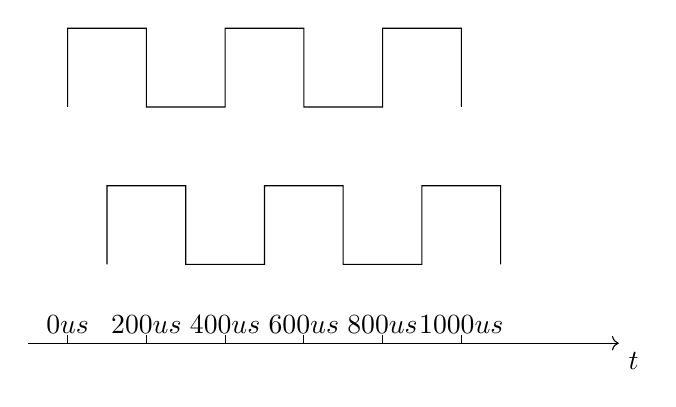
\begin{tikzpicture}[scale=1]

\coordinate (P) at (0.5, 0);
\coordinate (A) at (1, 0);
\coordinate (B) at (2, 0);
\coordinate (C) at (3, 0);
\coordinate (D) at (4, 0);
\coordinate (E) at (5, 0);
\coordinate (F) at (6, 0);
\coordinate (Q) at (8, 0);

\draw (A) node[above] {$0us$} -- ++(0, 3pt) ;
\draw (B) node[above] {$200us$} -- ++(0, 3pt);
\draw (C) node[above] {$400us$} -- ++(0, 3pt) ;
\draw (D) node[above] {$600us$} -- ++(0, 3pt) ;
\draw (E) node[above] {$800us$} -- ++(0, 3pt) ;
\draw (F) node[above] {$1000us$} -- ++(0, 3pt) ;

\draw[->] (P)--(Q) node [below right]{$t$};

\draw (1,3)
to[short] (1,4)
to[short] (2,4)
to[short] (2,3)
to[short] (3,3)
to[short] (3,4)
to[short] (4,4)
to[short] (4,3)
to[short] (5,3)
to[short] (5,4)
to[short] (6,4)
to[short] (6,3); 

\draw (1.5,1)
to[short] (1.5,2)
to[short] (2.5,2)
to[short] (2.5,1)
to[short] (3.5,1)
to[short] (3.5,2)
to[short] (4.5,2)
to[short] (4.5,1)
to[short] (5.5,1)
to[short] (5.5,2)
to[short] (6.5,2)
to[short] (6.5,1);

\end{tikzpicture}
\caption{正転の時のA相B相}
\end{center}
\end{figure}

正転の時、A相に対してB相が$  \pi/4 $遅れて出力されている.逆転の時、$  \pi/4 $進んで出力されている.さらに周期からこのDCモータが3000rpmで回転することがわかる.\\

\section{課題2}

モータの動作原理と,モータドライバの仕組みについて調べて説明してください.\\

\subsection{等価回路$ ^{[1]} $}

磁界中DCモータの構造は等価回路に置き換えて考えるのが一般的である.

\begin{figure}[h!]
    \centering
    \includegraphics[scale=0.4]{011.png}
    \caption{等価回路 }
\end{figure}

この回路で,Rはモータの電機子抵抗,Lはモータのインダクタンス,Cはコンデンサである.また,i(t)は電機子電流,T(t)は発生トルクを示す.\\

\subsection{等価回路に関する微分方程式$ ^{[1]} $}

いま,入力電圧$ e(t) $とする.等価回路に関する微分方程式は

	\begin{equation}
L\frac{di}{dt}+Ri(t)+\frac{1}{C}\int_{0}^{t}i(t)dt=e(t)
	\end{equation}
	
	
	今回の端電圧が$ v(t) $であるから,代入すると
	
	\begin{equation}
L\frac{di}{dt}+Ri(t)+v(t)=e(t)
	\end{equation}
	
	DCモータの逆起電力$ v(t) $とDCモータの回転速度は比例するであるから,
	
		\begin{equation}
v(t)=K_{E}\frac{d\theta}{dt}
	\end{equation}
	
	ここで$ K_{E} $は逆起電定数といい,さらに,発生トルク$ T(t) $は,トルク定数$ K_{T} $の間には,
	
	\begin{equation}
T(t)=K_{T}i(t)
	\end{equation}
	
	以上より,
	
	\begin{equation}
	L\frac{di}{dt}+R\frac{1}{K_{T}}T(t)+K_{E}\frac{d\theta}{dt}=e(t)
	\end{equation}
	
	慣性モーメントがJ,粘性摩擦係数がDの回転体にトルクがかかった出力側の回転運動方程式は下式のようになる.
	
	\begin{equation}
	J\frac{d\omega(t)}{dt}+D\omega(t)=T(t)
	\end{equation}
	
	
	\begin{equation}
	\frac{d\theta(t)}{dt}=\omega(t)
	\end{equation}


以上の方程式をラプラス変換を取って,入力$ \Omega(s) $から出力$ U(s) $までの一巡伝達関数は, 

\begin{equation}
	G(s)=\frac{\Omega(s)}{U(s)}=\frac{\frac{K_{T}}{R}\frac{1}{Js+D}}{1+\frac{K_{T}K_{E}}{R}\frac{1}{Js+D}}
	\end{equation}
	
	
	$ K=1,T=1 $でのステップ応答は以下のようになる.
	
	\newpage
	
	\begin{figure}[h!]
    \centering
    \includegraphics[scale=0.35]{015.jpeg}
    \caption{ステップ応答 }
\end{figure}

上の図のようになり, 定常値でKに, T秒後に最終値 K の 63.2\% に達すことがわかる.\\


\subsection{モータドライバの仕組$ ^{[3]} $}

モーター・ドライバとは,マイコンなどの制御部からの指示を受けてモーターを駆動,制御するためのデバイスである.
モーターを回転させるタイミングや速度を制御するにはマイコンは不可欠なデバイスである.しかし、マイコンの入出力ポートにはモーターを直接駆動できるほどのドライブ能力がないことがほとんどである.

この場合、制御するための信号をマイコンからモーター・ドライバに送り、モーター・ドライバを介して駆動する必要があある.


\newpage


\section{}
\begin{thebibliography}{9}
\bibitem{latexcompanion} 
JSMEテキストシリーズ  
[\textit{制御工学}]. 
 (2010/8/31),   p.19.20. 日本機械学会

\bibitem{latexcompanion} 
黒川一夫 
[\textit{ロボット用回路駆動設計}]. 
(2007/10/22),   p.4. 工学研究社


\bibitem{einstein} 
Embedded Technology Lab

[\textit{初心者こそ押さえておくべき!モーター・ドライバを使うべき理由}]. 
\url{https://lab.fujiele.co.jp/articles/7058/}



\end{thebibliography}





\end{document}